
%% bare_conf.tex
%% V1.3
%% 2007/01/11
%% by Michael Shell
%% See:
%% http://www.michaelshell.org/
%% for current contact information.
%%
%% This is a skeleton file demonstrating the use of IEEEtran.cls
%% (requires IEEEtran.cls version 1.7 or later) with an IEEE conference paper.
%%
%% Support sites:
%% http://www.michaelshell.org/tex/ieeetran/
%% http://www.ctan.org/tex-archive/macros/latex/contrib/IEEEtran/
%% and
%% http://www.ieee.org/

%%*************************************************************************
%% Legal Notice:
%% This code is offered as-is without any warranty either expressed or
%% implied; without even the implied warranty of MERCHANTABILITY or
%% FITNESS FOR A PARTICULAR PURPOSE! 
%% User assumes all risk.
%% In no event shall IEEE or any contributor to this code be liable for
%% any damages or losses, including, but not limited to, incidental,
%% consequential, or any other damages, resulting from the use or misuse
%% of any information contained here.
%%
%% All comments are the opinions of their respective authors and are not
%% necessarily endorsed by the IEEE.
%%
%% This work is distributed under the LaTeX Project Public License (LPPL)
%% ( http://www.latex-project.org/ ) version 1.3, and may be freely used,
%% distributed and modified. A copy of the LPPL, version 1.3, is included
%% in the base LaTeX documentation of all distributions of LaTeX released
%% 2003/12/01 or later.
%% Retain all contribution notices and credits.
%% ** Modified files should be clearly indicated as such, including  **
%% ** renaming them and changing author support contact information. **
%%
%% File list of work: IEEEtran.cls, IEEEtran_HOWTO.pdf, bare_adv.tex,
%%                    bare_conf.tex, bare_jrnl.tex, bare_jrnl_compsoc.tex
%%*************************************************************************

% *** Authors should verify (and, if needed, correct) their LaTeX system  ***
% *** with the testflow diagnostic prior to trusting their LaTeX platform ***
% *** with production work. IEEE's font choices can trigger bugs that do  ***
% *** not appear when using other class files.                            ***
% The testflow support page is at:
% http://www.michaelshell.org/tex/testflow/



% Note that the a4paper option is mainly intended so that authors in
% countries using A4 can easily print to A4 and see how their papers will
% look in print - the typesetting of the document will not typically be
% affected with changes in paper size (but the bottom and side margins will).
% Use the testflow package mentioned above to verify correct handling of
% both paper sizes by the user's LaTeX system.
%
% Also note that the "draftcls" or "draftclsnofoot", not "draft", option
% should be used if it is desired that the figures are to be displayed in
% draft mode.
%
\documentclass[10pt, conference, compsocconf]{IEEEtran}
% Add the compsocconf option for Computer Society conferences.
%
% If IEEEtran.cls has not been installed into the LaTeX system files,
% manually specify the path to it like:
% \documentclass[conference]{../sty/IEEEtran}





% Some very useful LaTeX packages include:
% (uncomment the ones you want to load)


% *** MISC UTILITY PACKAGES ***
%
%\usepackage{ifpdf}
% Heiko Oberdiek's ifpdf.sty is very useful if you need conditional
% compilation based on whether the output is pdf or dvi.
% usage:
% \ifpdf
%   % pdf code
% \else
%   % dvi code
% \fi
% The latest version of ifpdf.sty can be obtained from:
% http://www.ctan.org/tex-archive/macros/latex/contrib/oberdiek/
% Also, note that IEEEtran.cls V1.7 and later provides a builtin
% \ifCLASSINFOpdf conditional that works the same way.
% When switching from latex to pdflatex and vice-versa, the compiler may
% have to be run twice to clear warning/error messages.






% *** CITATION PACKAGES ***
%
%\usepackage{cite}
% cite.sty was written by Donald Arseneau
% V1.6 and later of IEEEtran pre-defines the format of the cite.sty package
% \cite{} output to follow that of IEEE. Loading the cite package will
% result in citation numbers being automatically sorted and properly
% "compressed/ranged". e.g., [1], [9], [2], [7], [5], [6] without using
% cite.sty will become [1], [2], [5]--[7], [9] using cite.sty. cite.sty's
% \cite will automatically add leading space, if needed. Use cite.sty's
% noadjust option (cite.sty V3.8 and later) if you want to turn this off.
% cite.sty is already installed on most LaTeX systems. Be sure and use
% version 4.0 (2003-05-27) and later if using hyperref.sty. cite.sty does
% not currently provide for hyperlinked citations.
% The latest version can be obtained at:
% http://www.ctan.org/tex-archive/macros/latex/contrib/cite/
% The documentation is contained in the cite.sty file itself.






% *** GRAPHICS RELATED PACKAGES ***
%
\usepackage[pdftex]{graphicx}
%\usepackage{graphicx}
\usepackage{epstopdf}
\usepackage{fancyvrb}
\ifCLASSINFOpdf
% \usepackage[pdftex]{graphicx}
  % declare the path(s) where your graphic files are
  % \graphicspath{{../pdf/}{../jpeg/}}
  % and their extensions so you won't have to specify these with
  % every instance of \includegraphics
  % \DeclareGraphicsExtensions{.pdf,.jpeg,.png}
\else
  % or other class option (dvipsone, dvipdf, if not using dvips). graphicx
  % will default to the driver specified in the system graphics.cfg if no
  % driver is specified.
  % \usepackage[dvips]{graphicx}
  % declare the path(s) where your graphic files are
  % \graphicspath{{../eps/}}
  % and their extensions so you won't have to specify these with
  % every instance of \includegraphics
  % \DeclareGraphicsExtensions{.eps}
\fi
% graphicx was written by David Carlisle and Sebastian Rahtz. It is
% required if you want graphics, photos, etc. graphicx.sty is already
% installed on most LaTeX systems. The latest version and documentation can
% be obtained at: 
% http://www.ctan.org/tex-archive/macros/latex/required/graphics/
% Another good source of documentation is "Using Imported Graphics in
% LaTeX2e" by Keith Reckdahl which can be found as epslatex.ps or
% epslatex.pdf at: http://www.ctan.org/tex-archive/info/
%
% latex, and pdflatex in dvi mode, support graphics in encapsulated
% postscript (.eps) format. pdflatex in pdf mode supports graphics
% in .pdf, .jpeg, .png and .mps (metapost) formats. Users should ensure
% that all non-photo figures use a vector format (.eps, .pdf, .mps) and
% not a bitmapped formats (.jpeg, .png). IEEE frowns on bitmapped formats
% which can result in "jaggedy"/blurry rendering of lines and letters as
% well as large increases in file sizes.
%
% You can find documentation about the pdfTeX application at:
% http://www.tug.org/applications/pdftex





% *** MATH PACKAGES ***
%
%\usepackage[cmex10]{amsmath}
% A popular package from the American Mathematical Society that provides
% many useful and powerful commands for dealing with mathematics. If using
% it, be sure to load this package with the cmex10 option to ensure that
% only type 1 fonts will utilized at all point sizes. Without this option,
% it is possible that some math symbols, particularly those within
% footnotes, will be rendered in bitmap form which will result in a
% document that can not be IEEE Xplore compliant!
%
% Also, note that the amsmath package sets \interdisplaylinepenalty to 10000
% thus preventing page breaks from occurring within multiline equations. Use:
%\interdisplaylinepenalty=2500
% after loading amsmath to restore such page breaks as IEEEtran.cls normally
% does. amsmath.sty is already installed on most LaTeX systems. The latest
% version and documentation can be obtained at:
% http://www.ctan.org/tex-archive/macros/latex/required/amslatex/math/





% *** SPECIALIZED LIST PACKAGES ***
%
%\usepackage{algorithmic}
% algorithmic.sty was written by Peter Williams and Rogerio Brito.
% This package provides an algorithmic environment fo describing algorithms.
% You can use the algorithmic environment in-text or within a figure
% environment to provide for a floating algorithm. Do NOT use the algorithm
% floating environment provided by algorithm.sty (by the same authors) or
% algorithm2e.sty (by Christophe Fiorio) as IEEE does not use dedicated
% algorithm float types and packages that provide these will not provide
% correct IEEE style captions. The latest version and documentation of
% algorithmic.sty can be obtained at:
% http://www.ctan.org/tex-archive/macros/latex/contrib/algorithms/
% There is also a support site at:
% http://algorithms.berlios.de/index.html
% Also of interest may be the (relatively newer and more customizable)
% algorithmicx.sty package by Szasz Janos:
% http://www.ctan.org/tex-archive/macros/latex/contrib/algorithmicx/




% *** ALIGNMENT PACKAGES ***
%
%\usepackage{array}
% Frank Mittelbach's and David Carlisle's array.sty patches and improves
% the standard LaTeX2e array and tabular environments to provide better
% appearance and additional user controls. As the default LaTeX2e table
% generation code is lacking to the point of almost being broken with
% respect to the quality of the end results, all users are strongly
% advised to use an enhanced (at the very least that provided by array.sty)
% set of table tools. array.sty is already installed on most systems. The
% latest version and documentation can be obtained at:
% http://www.ctan.org/tex-archive/macros/latex/required/tools/


%\usepackage{mdwmath}
%\usepackage{mdwtab}
% Also highly recommended is Mark Wooding's extremely powerful MDW tools,
% especially mdwmath.sty and mdwtab.sty which are used to format equations
% and tables, respectively. The MDWtools set is already installed on most
% LaTeX systems. The lastest version and documentation is available at:
% http://www.ctan.org/tex-archive/macros/latex/contrib/mdwtools/


% IEEEtran contains the IEEEeqnarray family of commands that can be used to
% generate multiline equations as well as matrices, tables, etc., of high
% quality.


%\usepackage{eqparbox}
% Also of notable interest is Scott Pakin's eqparbox package for creating
% (automatically sized) equal width boxes - aka "natural width parboxes".
% Available at:
% http://www.ctan.org/tex-archive/macros/latex/contrib/eqparbox/





% *** SUBFIGURE PACKAGES ***
%\usepackage[tight,footnotesize]{subfigure}
% subfigure.sty was written by Steven Douglas Cochran. This package makes it
% easy to put subfigures in your figures. e.g., "Figure 1a and 1b". For IEEE
% work, it is a good idea to load it with the tight package option to reduce
% the amount of white space around the subfigures. subfigure.sty is already
% installed on most LaTeX systems. The latest version and documentation can
% be obtained at:
% http://www.ctan.org/tex-archive/obsolete/macros/latex/contrib/subfigure/
% subfigure.sty has been superceeded by subfig.sty.



%\usepackage[caption=false]{caption}
\usepackage[font=footnotesize]{subfig}
% subfig.sty, also written by Steven Douglas Cochran, is the modern
% replacement for subfigure.sty. However, subfig.sty requires and
% automatically loads Axel Sommerfeldt's caption.sty which will override
% IEEEtran.cls handling of captions and this will result in nonIEEE style
% figure/table captions. To prevent this problem, be sure and preload
% caption.sty with its "caption=false" package option. This is will preserve
% IEEEtran.cls handing of captions. Version 1.3 (2005/06/28) and later 
% (recommended due to many improvements over 1.2) of subfig.sty supports
% the caption=false option directly:
%\usepackage[caption=false,font=footnotesize]{subfig}
%
% The latest version and documentation can be obtained at:
% http://www.ctan.org/tex-archive/macros/latex/contrib/subfig/
% The latest version and documentation of caption.sty can be obtained at:
% http://www.ctan.org/tex-archive/macros/latex/contrib/caption/




% *** FLOAT PACKAGES ***
%
%\usepackage{fixltx2e}
% fixltx2e, the successor to the earlier fix2col.sty, was written by
% Frank Mittelbach and David Carlisle. This package corrects a few problems
% in the LaTeX2e kernel, the most notable of which is that in current
% LaTeX2e releases, the ordering of single and double column floats is not
% guaranteed to be preserved. Thus, an unpatched LaTeX2e can allow a
% single column figure to be placed prior to an earlier double column
% figure. The latest version and documentation can be found at:
% http://www.ctan.org/tex-archive/macros/latex/base/



%\usepackage{stfloats}
% stfloats.sty was written by Sigitas Tolusis. This package gives LaTeX2e
% the ability to do double column floats at the bottom of the page as well
% as the top. (e.g., "\begin{figure*}[!b]" is not normally possible in
% LaTeX2e). It also provides a command:
%\fnbelowfloat
% to enable the placement of footnotes below bottom floats (the standard
% LaTeX2e kernel puts them above bottom floats). This is an invasive package
% which rewrites many portions of the LaTeX2e float routines. It may not work
% with other packages that modify the LaTeX2e float routines. The latest
% version and documentation can be obtained at:
% http://www.ctan.org/tex-archive/macros/latex/contrib/sttools/
% Documentation is contained in the stfloats.sty comments as well as in the
% presfull.pdf file. Do not use the stfloats baselinefloat ability as IEEE
% does not allow \baselineskip to stretch. Authors submitting work to the
% IEEE should note that IEEE rarely uses double column equations and
% that authors should try to avoid such use. Do not be tempted to use the
% cuted.sty or midfloat.sty packages (also by Sigitas Tolusis) as IEEE does
% not format its papers in such ways.





% *** PDF, URL AND HYPERLINK PACKAGES ***
%
%\usepackage{url}
% url.sty was written by Donald Arseneau. It provides better support for
% handling and breaking URLs. url.sty is already installed on most LaTeX
% systems. The latest version can be obtained at:
% http://www.ctan.org/tex-archive/macros/latex/contrib/misc/
% Read the url.sty source comments for usage information. Basically,
% \url{my_url_here}.





% *** Do not adjust lengths that control margins, column widths, etc. ***
% *** Do not use packages that alter fonts (such as pslatex).         ***
% There should be no need to do such things with IEEEtran.cls V1.6 and later.
% (Unless specifically asked to do so by the journal or conference you plan
% to submit to, of course. )


% correct bad hyphenation here
\hyphenation{op-tical net-works semi-conduc-tor}


\begin{document}
%
% paper title
% can use linebreaks \\ within to get better formatting as desired
\title{iMonitor: An Implicit-Signal Monitor}


% author names and affiliations
% use a multiple column layout for up to two different
% affiliations

\author{\IEEEauthorblockN{Wei-Lun Hung and Vijay K. Garg}
\IEEEauthorblockA{Department of Electrical and Computer Engineering \\
The University of Texas at Austin \\
Austin, TX 78712-1084, USA \\
wlhung@utexas.edu, garg@ece.utexas.edu}
}

% conference papers do not typically use \thanks and this command
% is locked out in conference mode. If really needed, such as for
% the acknowledgment of grants, issue a \IEEEoverridecommandlockouts
% after \documentclass

% for over three affiliations, or if they all won't fit within the width
% of the page, use this alternative format:
% 
%\author{\IEEEauthorblockN{Michael Shell\IEEEauthorrefmark{1},
%Homer Simpson\IEEEauthorrefmark{2},
%James Kirk\IEEEauthorrefmark{3}, 
%Montgomery Scott\IEEEauthorrefmark{3} and
%Eldon Tyrell\IEEEauthorrefmark{4}}
%\IEEEauthorblockA{\IEEEauthorrefmark{1}School of Electrical and Computer Engineering\\
%Georgia Institute of Technology,
%Atlanta, Georgia 30332--0250\\ Email: see http://www.michaelshell.org/contact.html}
%\IEEEauthorblockA{\IEEEauthorrefmark{2}Twentieth Century Fox, Springfield, USA\\
%Email: homer@thesimpsons.com}
%\IEEEauthorblockA{\IEEEauthorrefmark{3}Starfleet Academy, San Francisco, California 96678-2391\\
%Telephone: (800) 555--1212, Fax: (888) 555--1212}
%\IEEEauthorblockA{\IEEEauthorrefmark{4}Tyrell Inc., 123 Replicant Street, Los Angeles, California 90210--4321}}




% use for special paper notices
%\IEEEspecialpapernotice{(Invited Paper)}




% make the title area
\maketitle


\begin{abstract}
The abstract goes here. DO NOT USE SPECIAL CHARACTERS, SYMBOLS, OR MATH IN YOUR TITLE OR ABSTRACT.

\end{abstract}

\begin{IEEEkeywords}
automatic signal, concurrency, explicit signal, implicit signal,
monitor, parallel

\end{IEEEkeywords}


% For peer review papers, you can put extra information on the cover
% page as needed:
% \ifCLASSOPTIONpeerreview
% \begin{center} \bfseries EDICS Category: 3-BBND \end{center}
% \fi
%
% For peerreview papers, this IEEEtran command inserts a page break and
% creates the second title. It will be ignored for other modes.
\IEEEpeerreviewmaketitle



\section{Introduction} \label{sec:intro}
% no \IEEEPARstart
Developing efficient and robust concurrent programs within a limited time is 
critical than ever. On the one hand, the multi-core processor, which allows 
multiple threads to be executed at the same time, has become the mainstream of 
computers; however, the power of multi-core processors is limited due to the 
lack of concurrent applications. On the other hand, to compete with other rivals
and to satisfy consumer demands in software industry, an application needs to be
developed quickly. The concurrent programming is 
different from the traditional sequential programming. Multiple threads may 
interact with each other and try to access the same source. Therefore, providing
correctness of current programs is more difficult than sequential programs. In 
addition, the debugging process is panic in concurrent programs due to the 
thread scheduling. 

The monitor \cite{hoa74} is commonly used in concurrent programming for 
maintaining the mutual exclusion of shared resources and providing the 
synchronization mechanism between threads. Buhr and Harji \cite{bh05} divide 
monitors into two categories, the explicit-signal monitor and the 
implicit-signal monitor. Buhr and Harji use the explicit-signal monitor to 
simulate the implicit-signal monitor and point out that the implicit-signal 
monitor is not as efficient as the explicit-signal monitor. However, the 
implicit-signal is easy to be used and useful in concurrent programming,
especially for prototyping. 


Most programming languages, including the popular object-oriented language Java,
only provide the explicit-signal monitor but not implicit-signal. This research 
focuses on developing a framework supporting implicit-signal monitor without
sacrificing efficiency in the modern programming language - Java. 

our contribution

This paper is organized as follows. Section \ref{sec:pre} gives the
preliminaries. 
Our framework is presented in Section \ref{sec:fw} and the practical 
implementation details are discussed in Section \ref{sec:imp}. The proposed 
methods are then evaluated with experiments in Section \ref{sec:eval}. 
Section \ref{sec:conclu} gives the concluding remarks.
% You must have at least 2 lines in the paragraph with the drop letter
% (should never be an issue)

\section{Preliminaries} \label{sec:pre}
\subsection{Predicate}
A predicate which depends on some variables is a statement that is either true
or false. For example, $x > 0$ is a predicate where x is an integer variable. 
Predicates are commonly used to describe the properties of conditions. 
Predicates can be divided into two categories based on their variables.
\subsubsection{Global predicate} A predicate contains only shared variables of a
    monitor. 
\subsubsection{Local predicate} If both shared variables and local variables of a
    member function are in the predicate, which is called local predicate. 

\subsection{Monitor}
Monitor is an abstract object or module containing shared data to be used safely
by multiple member functions and threads in concurrent programming. Monitor can
be defined by two characteristics, mutual exclusion and synchronization. Mutual 
exclusion guarantees that at most one thread can execute any member function of 
a monitor at each time. The mutual exclusion provides programmers a more elegant
way to update shared data compared to directly accessing shared date. 
Synchronization maintains the executing order between threads. Threads may wait
for some condition to be met and release mutual exclusion temporarily. After the
condition has met, threads then re-acquire mutual exclusion and continue to 
execute.
According to Buhr and Harji \cite{bh05}, monitors can be divided into two 
categories based on the difference implementations of synchronization. 
  \subsubsection{Explicit-signal monitor} In this type of monitor, conditional
    variables
    and signal/await statement are used for synchronization. Programmers need to
    associate assertions with conditional variables manually. The mechanism of
    synchronization is achieved by two threads. One tread checks if some
    assertion is met or not and then explicit await if the assertion is not
    met. When another thread detects the state has changed and the assertion is
    met, and then explicitly signals appropriate threads in the monitor.
  \subsubsection{Implicit-signal monitor} This kind of monitor uses waituntil
    statements instead of conditional variables for
    synchronization. Programmers do not need to associate assertions with
    variables but use waituntil statements and logical predicate directly. In
    this kind of monitor, a thread will wait if the predicate of a waitutil
    statement is false, and execute the remaining tasks after the predicate
    has become true automatically.

Explicit-signal and implicit-signal monitors have different pros and cons. The 
explicit-signal has more complex syntax than the implicit-signal monitor. In 
addition, the explicit-signal needs the programmers to write the synchronization
mechanism manually, which increases the chance of writing incorrect code. 
However, in practice, explicit-signal is more efficient than implicit-signal. 
The implicit-signal monitor is still useful in prototyping and verification. 
Nevertheless, most of modern programming languages do not provide the 
implicit-signal monitor mechanism.




\subsection{Motivations for Implicit-Signal Monitor}
The concurrent programs are more difficult to be written and debugged than the 
sequential programs. Although explicit-signal monitor already provides an 
elegant mechanism for programmers to maintain mutual exclusion and synchronization 
in concurrent programs; implicit-signal is more straightforward in both code
reasoning and syntax. 

Fig.~\ref{fig:bb_exp} shows an example to
demonstrate the difference between implicit-signal monitor and explicit-signal 
monitor. The problem is producer-consumer problem, also known as bounded-buffer
problem. There are two kinds of threads, producers and consumers, which are 
trying to obtain access to the shared resources. Producers try to put items 
into the buffer and consumers try to take items out from the buffer. Every 
operation should be mutual exclusion. In addition, a producer cannot put any 
item when the buffer is full and a consumer cannot take any item when the 
buffer is empty. Fig.~\ref{subfig:bb_exam_exp} is written by the original Java
program language. A lock variable and conditional variables are
needed to maintain mutual exclusion and synchronization. A thread needs to
acquire the lock before entering member functions. In addition, programmers need
to explicitly associate the assertions with conditional variables and call
signal/await statement manually. Fig.~\ref{subfig:bb_exam_imp} shows a Java-alike
program for the producer-consumer problem. The key word $monitor$ for $class$
indicates that every member function of the class can only be executed at most
one thread at any time. In addition, the $waituntil$ statement indicates that if
the predicate of the waituntil is not true, the executing thread must wait and
release the monitor temporarily. After the predicate becomes true, the thread
then can awake automatically. As can be seen, Fig.~\ref{subfig:bb_exam_imp} is
more straightforward and simpler than Fig.~\ref{subfig:bb_exam_exp}. This research
focuses on developing a framework supporting such java-alike language without 
sacrificing efficiency.


\begin{SaveVerbatim}{OriginBoundedBuffer}
class BoundedBuffer {
  Object[] items;  
  lock mutex;
  condition notFull, notEmpty;
  int putPtr, takePtr, count;
  public void put(Object x) {
    mutex.lock();
    if(count == items.length) {
      notFull.await();
    }
    items[putPtr] = x;
    if(++putPtr == items.length) {
      putPtr = 0;
    }
    ++count;
    notEmpty.signal();
    mutex.unlock();
  }
  public Object take() {
    mutex.lock();
    if(count == 0) {
      notEmpty.await();
    }
    int x = items[takePtr];
    if(++takePtr == items.length) {
      takePtr = 0;
    }
    --count;
    notFull.signal();
    mutex.unlock();
    return x;
  }
}
\end{SaveVerbatim}

\begin{SaveVerbatim}{iMonitorBoundedBuffer}
monitor class BoundedBuffer { 
  Object[] items; 
  int putPtr, takePtr, count; 
  public void put(Object x) { 
    waituntil(count < items.length); 
    items[putPtr] = x; 
    if(++putPtr == items.length) { 
      putPtr = 0; 
    } 
    ++count; 
  } 
  public Object take() { 
    waituntil(count > 0); 
    Object x = items[takePtr]; 
    if(++takePtr == items.length) { 
      takePtr = 0; 
    }
    --count;
    return x;
  }
}
\end{SaveVerbatim}

\begin{figure}
  \centering
  \subfloat[Explicit-Signal] {
    \fbox{
      \BUseVerbatim[fontsize=\footnotesize]{OriginBoundedBuffer}
    }
    \label{subfig:bb_exam_exp}
  }
  \\
  \subfloat[Implicit-Signal] {
    \fbox{
      \BUseVerbatim[fontsize=\footnotesize]{iMonitorBoundedBuffer}
    }
    \label{subfig:bb_exam_imp}
  }
  \caption{Bounded-buffer example}
  \label{fig:bb_exp}
\end{figure}


\section{Framework of iMonitor} \label{sec:fw}
To make the implicit-signal available in the modern high-level language, Java, 
the iMonitor framework is proposed. Fig.~\ref{fig:framework} illustrates the 
framework of the iMonitor. The iMonitor takes a Java-extension program providing
the implicit-signal mechanism through supporting monitor class and waituntil 
statement. The iMonitor preprocessor transfers the iMonitor code into the 
tradition Java code which can be compiled with iMonitor library. The iMonitor 
Java library implements different kinds of implicit-signal monitor mechanisms. 
Programmers may choose one mechanism which is the most efficient for their 
requirements by providing some parameters to the preprocessor. Rewriting 
programs is unnecessary for different approaches of implicit-signal monitors. 
The flexibility is provided without any additional cost. 

\begin{figure}[ht!]
  \centering
  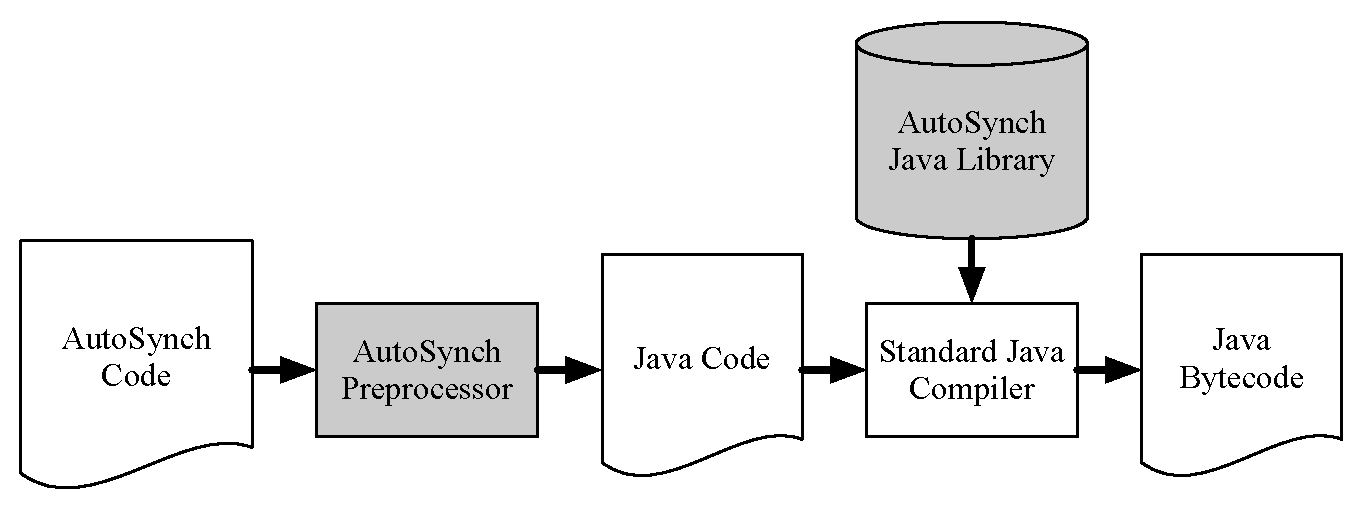
\includegraphics[width=80mm]{fig/flow.eps}
  \caption{The framework of iMonitor}
  \label{fig:framework}
\end{figure}

\section{Desirable Properties}
\subsection{Every thread can check predicates}
\subsection{Less predicates need to be checked}
\subsection{Reduce the number of content switch}

\section{Enabling Techniques}

\subsection{Globalization}
An operation called globalization is defined as replacing all local variables of
a predicate by its values at the time. The globalization converts a local 
predicate into a global predicate since all the local variables have been 
replaced. The globalization has an important characteristic that allows a
local predicate to be evaluated by any other thread safely after the original
thread waits. Since no other thread can access to local variables of a member 
function in which a particular thread is executing, values of local variables 
cannot be changed by other threads after the particular thread is waiting. 
Therefore, all other threads can check the globalized predicate safely. 


\subsection{Equivalence Predicate Reduction}

\subsection{Remove Local Predicate pairs as soon as possible}

\subsection{Only one executable thread is signaled}
reduce the number of content switch and the number of predicate checking 


\section{Practical Implementation} \label{sec:imp}
The implementation of the implicit-signal monitor in iMonitor involves four 
parts:
\begin{enumerate}
  \item Monitor-constructor: the constructor of the monitor class, including 
    definitions and declarations of additional variables to provide mutual 
    exclusion and synchronization of monitor. 
  \item Monitor-function entry: executed before each member function, 
    involving declarations of additional variables and code to maintain
    mutual exclusion of monitor. 
  \item Monitor-waituntil statement: including declarations of additional
    variables and signal/await statements to implement the waituntil.
  \item Monitor-function leave: executed before the return statement of 
    each member function, involving code to guarantee mutual exclusion and 
    synchronization of monitor. 
\end{enumerate}
%I would like to use Table \ref{tab:constructor_imp},
%\ref{tab:entry_imp}, \ref{tab:waituntilc_imp} and \ref{tab:exit_imp} to sumarize
%the implementations of different kinds of implicit-signal monitors. 



\subsection{Naive}

\begin{SaveVerbatim}{NaiveConstructorImp}

Lock L;
Condition C;
\end{SaveVerbatim}

\begin{SaveVerbatim}{NaiveEntryImp}

lock L 
\end{SaveVerbatim}

\begin{SaveVerbatim}{NaiveWaituntilImp}

if P is false
  signal all C
  do 
    wait C
  while P is false
\end{SaveVerbatim}

\begin{SaveVerbatim}{NaiveExitImp}

signal all C
unlock L
\end{SaveVerbatim}

\begin{SaveVerbatim}{NConditionConstructorImp}

Lock L
List<Predicate, Condition> LIST
foreach global predicate P
  create a pair <P, C>
  add <P, C> to LIST
\end{SaveVerbatim}

%\begin{SaveVerbatim}{NConditionWaituntilImp}
%if P is a local predicate 
%  create a pair <P, C>
%  add <P, C> to LIST
% 
%if P is false 
%  foreach <PI, CI> in LIST
%    if PI is true
%      signal CI
%  do 
%    wait C
%  while P is false
%
%if P is a local predicate 
%  remove <P, C> from LIST
%\end{SaveVerbatim}
%
%\begin{SaveVerbatim}{NConditionExitImp}
%foreach <P, C> in LIST
%  if P is true
%    signal C
%
%unlock L
%\end{SaveVerbatim}


\begin{SaveVerbatim}{MapConditionConstructorImp}

Lock L
Map<Predicate, Condition> MAP
foreach global predicate P
  if P is not in MAP
    create a pair <P, C>
    add <P, C> to MAP 
\end{SaveVerbatim}

\begin{SaveVerbatim}{MapConditionWaituntilImp}

if P is a local predicate 
  PE := Globalization(P)
  if PE is not in MAP
    create a pair <PE, C>
    add <PE, C> to MAP
 
if P is false 
  foreach <PI, CI> in MAP
    if PI is true and CI has waiter
      signal CI
      break
  do 
    wait C
  while P is false

if P is local predicate 
    and C has no waiter
  remove <PE, C> from MAP
\end{SaveVerbatim}

\begin{SaveVerbatim}{MapConditionExitImp}

foreach <P, C> in MAP
  if P is true and C has waiter
    signal C
    break
unlock L
\end{SaveVerbatim}


%\begin{table*}
%  \center
%  \begin{tabular}{| l || l | l | }
%    \hline
%    Naive & \BUseVerbatim{NaiveConstructorImp} \\
%                
%    \hline
%    N-Condition & \BUseVerbatim{NConditionConstructorImp} \\
%    \hline
%    Map & \BUseVerbatim{MapConditionConstructorImp} \\
%    \hline
%  \end{tabular}
%  \caption{iMonitor implementation(Contructor)}
%  \label{tab:constructor_imp}
%\end{table*}
%
%\begin{table*}
%  \center
%  \begin{tabular}{| l || l |}
%    \hline
%    Naive & \BUseVerbatim{NaiveEntryImp} \\
%                
%    \hline
%    N-Condition & \BUseVerbatim{NaiveEntryImp} \\
%    \hline
%    Map & \BUseVerbatim{NaiveEntryImp} \\
%    \hline
%  \end{tabular}
%  \caption{iMonitor implementation(Entry)}
%  \label{tab:entry_imp}
%\end{table*}
%
%\begin{table*}
%  \center
%  \begin{tabular}{| l || l |}
%    \hline
%    Naive & \BUseVerbatim{NaiveWaituntilImp} \\
%                
%    \hline
%    N-Condition & \BUseVerbatim{NConditionWaituntilImp} \\
%    \hline
%    Map & \\
%    \hline
%  \end{tabular}
%  \caption{iMonitor implementation(Waituntil C)}
%  \label{tab:waituntilc_imp}
%\end{table*}
%
%\begin{table*}
%  \center
%  \begin{tabular}{| l || l |}
%    \hline
%    Naive & \BUseVerbatim{NaiveExitImp} \\
%                
%    \hline
%    N-Condition & \BUseVerbatim{NConditionExitImp} \\
%    \hline
%    Map & \BUseVerbatim{MapConditionExitImp} \\
%    \hline
%  \end{tabular}
%  \caption{iMonitor implementation(Exit)}
%  \label{tab:exit_imp}
%\end{table*}


In the implementation of naive implicit-signal monitor, one lock variable, 
$L$, is declared for mutual exclusion, which should be acquired in 
the beginning of every member function and released before the return statement.
In addition, one conditional variable, $C$, is declared for 
synchronization, on which the implementation of waituntil depends. In the 
waituntil statement, the predicate expression is checked initially. If the 
expression is false; then all other threads which are waiting on $C$ are 
signaled to reevaluate their predicate expression since the monitor state may 
change. The current thread then is blocked in a loop and reevaluates its 
predicate expression when it is signaled. On the exit of a member function, 
all threads waiting on $C$ are signaled to reevaluate their predicate 
expression since the monitor state may change. Table \ref{tab:imp_naive} 
summarize the implementation of naive implicit-signal monitor. Although 
the naive implicit-signal monitor is easy to implement, it is inefficient. 
When a predicate is evaluated as false or a thread want to leave the monitor, 
all other threads waiting one the same monitor will be awaked and need to 
recheck their conditions.

\begin{table}
    \center
    \begin{tabular}{|l|l|} 
      \hline
      Constructor & \BUseVerbatim[baselinestretch=1.1]{NaiveConstructorImp}\\
      \hline
      Enter & \BUseVerbatim[baselinestretch=1.1]{NaiveEntryImp}\\
      \hline
      Waituntil $P$ & \BUseVerbatim[baselinestretch=1.1]{NaiveWaituntilImp}\\
      \hline
      Exit & \BUseVerbatim[baselinestretch=1.1]{NaiveExitImp} \\
      \hline
    \end{tabular}
    \caption{The naive implicit-signal monitor implementation}
    \label{tab:imp_naive}
\end{table}

%\subsection{N-Condition}
%Instead of using only one conditional variable for synchronization, the 
%N-condition implicit-signal monitor uses multiple conditional variables.
%Every predicate in a waituntial statement has an associating conditional variable.
%The pair of a predicate assertion and a conditional variable is stored in a shared list, 
%$LIST$. For each global predicate, a pair of a predicate and a conditional 
%variable is created in the constructor. In the waituntil statement, the type of 
%predicate is checked. If the predicate is local predicate, then a corresponding 
%conditional variable is created and stored. The predicate expression is then 
%checked. If the predicate is false, threads which waits on some true predicates 
%are signaled. The current thread then is blocked and recheck 
%the predicate expression when it is signaled. After the predicate becomes
%true, the pair of predicate and conditional variable is removed from the 
%$LIST$ if the predicate ls local predicate. When a thread finishes jobs and wants
%to leave the monitor, the list of predicates are checked. Thread which wait 
%on a true predicate are signaled. Table \ref{tab:imp_n_cond} summarized the 
%implementation. Note that, only threads waiting on the true predicates are
%signaled. Therefore, the number
%of unnecessary signals and predicate checking is reduced. Moreover, it prevents programmers form abusing
%signalAll statement in explicit-signal monitor. However,  when a thread 
%executes the waituntil statement, 
%a conditional variable is created for a local predicate. It is extremely 
%expensive when waituntil statements with local predicates are executed many
%times.
%% remove signal all 
%
%\begin{table}
%    \center
%    \begin{tabular}{|l|l|} 
%      \hline
%      Constructor & \BUseVerbatim{NConditionConstructorImp}\\
%      \hline
%      Enter & \BUseVerbatim{NaiveEntryImp}\\
%      \hline
%      Waituntil $P$ & \BUseVerbatim{NConditionWaituntilImp}\\
%      \hline
%      Exit & \BUseVerbatim{NConditionExitImp} \\
%      \hline
%    \end{tabular}
%    \caption{The N-condition implicit-signal monitor implementation}
%    \label{tab:imp_n_cond}
%\end{table}

\subsection{Map-Condition}
The map-condition predicate uses the data structure map to store pairs of 
predicate and conditional variables. A predicate and a corresponding conditional
variable are treated as key and value respectively. For every global predicate, 
a corresponding conditional variable is created and the pair of a predicate and a
conditional variable is added to the map in the constructor. For every local 
predicate, the globalization has been applied to the local 
predicate. Every local variable is replaced in the local predicate by its value
at this point. The globalization does not affect on the results of 
predicate evaluations since other threads cannot change the value of local 
variables but only global variables. After applying globalization to
the local predicate, a new predicate with only global variable is derived. 
If the predicate has not been added to the shared map, then the new 
predicated is added to the map with a corresponding conditional variable.
Otherwise, the corresponding conditional variable can be found by searching the
predicate in the map. Hence, the number of creating and removing conditional
variables has been reduced. 


\begin{table}
    \center
    \begin{tabular}{|l|l|} 
      \hline
      Constructor & \BUseVerbatim[baselinestretch=1.1]{MapConditionConstructorImp}\\
      \hline
      Enter & \BUseVerbatim[baselinestretch=1.1]{NaiveEntryImp}\\
      \hline
      Waituntil $P$ & \BUseVerbatim[baselinestretch=1.1]{MapConditionWaituntilImp}\\
      \hline
      Exit & \BUseVerbatim[baselinestretch=1.1]{MapConditionExitImp} \\
      \hline
    \end{tabular}
    \caption{The map-condition implicit-signal monitor implementation}
    \label{tab:imp_map_cond}
\end{table}

\section{Evaluations} \label{sec:eval}
%\subsection{Saturation}
Four kinds of experiments were performed to evaluate the performances of the
explicit-signal monitor with original Java and the implicit-signal monitor with
iMonitor framework. All of the experiments were conducted on a machine with 16 
Intel(R) Xeon(R) X5560 CPUs and 64 GBs memory. 


Fig.~\ref{fig:pc_eval} shows the results of producer-consumer problem. The
x-axis indicates the number of producers and consumers; the y-axis indicates the
runtime in seconds. Total 512000 $put$ and $take$ operations were executed by
all producers and consumers. As expected, the naive approach is much slower than
others. Both N-Condition and map approaches are slightly slower in most cases.
This phenomenon can be explained as follows. Observe explicit-signal and 
implicit-signal approaches for the producer-consumer problem is shown in 
Fig.~\ref{fig:bb_exp}. In the implicit-signal approaches, there are only two 
waituntil statements with global predicates, $count > 0$ and 
$count < items.length$. In the naive approach, producers and consumers are
signaled every time when a thread await or want to leave the monitor. Therefore,
if a consumer waits because $count = 0$, all other consumers are awaken and
check the predicate $count > 0$. Such kind of operations is redundant and lead
to the inefficiency of naive implementation. The map
implementations only need to check two global predicates in a waituntil
statement and the exit of monitor. Hence, the N-Condition and map implementation 
has the similar performance and only slightly slower than the explicit-signal
monitor approach. 
\begin{figure}[ht!]
  \centering
  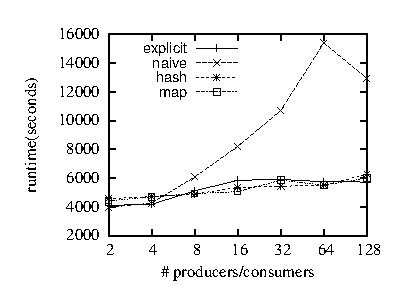
\includegraphics[width=80mm]{fig/pc.eps}
  \caption{The results of producer-consumer problem}
  \label{fig:pc_eval}
\end{figure}

\begin{SaveVerbatim}{OriginRandomBoundedBuffer}
class BoundedBuffer {
  Object[] items;  
  lock mutex;
  condition noSufficientSpace;
  condition noSufficientItem;
  int putPtr, takePtr, count;
  public void put(int n) {
    mutex.lock();
    while(n + count > items.length) {
      noSufficientSpace.await();
    }
    for(int i = 0; i < n; ++i) {
      items[putPtr++] = new Object();
      if(putPtr == items.length) {
        putPtr = 0;
      }
    }
    count += n;
    noSufficientItem.signalAll();
    mutex.unlock();
  }
  public Object[] take(int n) {
    mutex.lock();
    while(count < n) {
      noSufficientItem.await();
    }
    Object[] ret = new Object[n];
    for(int i = 0; i < n; ++i) {
      ret[i] = items[takePtr++];
      if(takePtr == items.length) {
        takePtr = 0;
      }
    }
    count -= n;
    noSufficientSpace.signalAll();
    mutex.unlock();
    return ret;
  }
}
\end{SaveVerbatim}

\begin{SaveVerbatim}{iMonitorRandomBoundedBuffer}
monitor class BoundedBuffer { 
  Object[] items; 
  int putPtr, takePtr, count; 
  public void put(int n) { 
    waituntil(count + n <= items.length); 
    for(int i = 0; i < n; ++i) {
      items[putPtr++] = new Object(); 
      if(putPtr == items.length) { 
        putPtr = 0; 
      } 
    }
    count += n; 
  } 
  public Object[] take(int n) { 
    waituntil(count >= n);
    Object[] ret = new Object[n];
    for(int i = 0; i < n; ++i) {
      ret[i] = items[takePtr++]; 
      if(takePtr == items.length) { 
        takePtr = 0; 
      }
    }
    count -= n;
    return ret;
  }
}
\end{SaveVerbatim}

\begin{figure}
  \centering
  \subfloat[Explicit-Signal] {
    \fbox{
      \BUseVerbatim[fontsize=\footnotesize]{OriginRandomBoundedBuffer}
    }
    \label{subfig:rbb_exam_exp}
  }
  \\
  \subfloat[Implicit-Signal] {
    \fbox{
      \BUseVerbatim[fontsize=\footnotesize]{iMonitorRandomBoundedBuffer}
    }
    \label{subfig:rbb_exam_imp}
  }
  \caption{Random Bounded-buffer example}
  \label{fig:rbb_exp}
\end{figure}
\begin{figure}[ht!]
  \centering
  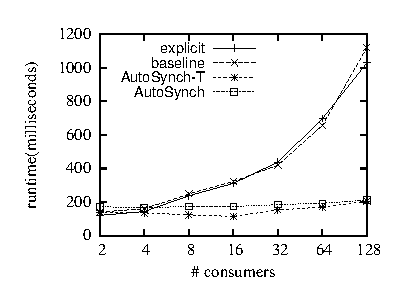
\includegraphics[width=80mm]{fig/rpc.eps}
  \caption{The results of random producer-consumer problem}
  \label{fig:rpc_eval}
\end{figure}

%Fig.~\ref{fig:rw_eval} shows the results of reader-writer problem. The
%x-axis indicates the number of readers and writers; the y-axis indicates the
%runtime in seconds. Total 1280 read/write operations were executed by all
%readers and writers. Since readers can read with each other at the same time.
%The runtime decreases as number of readers increases. Need to figure out why 
%explicit-signal approach is so slow in 1/5. Maybe the implementation? 
%
%\begin{figure}[ht!]
%  \centering
%  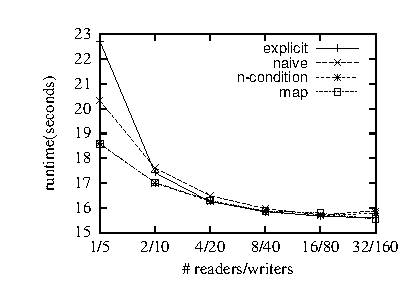
\includegraphics[width=80mm]{fig/rw.eps}
%  \caption{The results of reader-writer problem}
%  \label{fig:rw_eval}
%\end{figure}


%The dining philosophers problem is often used in computer science to describe 
%the synchronization issues. There are N philosophers siting around at a table 
%with a dish in front of them and a chopstick in between each philosopher. A 
%philosopher only think or eat. A philosopher needs to pick two chopsticks at the
%same time for eating and he does not put down a chopstick until he finishes 
%eating. If the chopstick is hold by another philosopher, then the philosopher 
%who want to eat must wait. In addition, a philosopher cannot eat forever, which
%means he will put down chopstick eventually. Every philosopher must be able to
%eat eventually if he is hungry. Figure 3. illustrate the experimental results
%of the dining philosophers problem. The x-axis depicts the runtime and the 
%y-axis describes the number of philosophers. As can be seen, three approaches 
%has the similar results. The implementations of Naive and N-condition are as 
%efficient as the implementation of explicit signal monitor. 
%
Fig.~\ref{fig:rr_eval} shows the results of round-robin access pattern. The
x-axis indicates the number of threads; the y-axis indicates the
runtime in seconds. In this set of experiments, threads are allowed to enter a
monitor in round-robin scheduling. Again, the results of N-Condition approach
are not shown because their performance is much worse than others. Total 
128000 operations were performed on the monitor. In this set
of experiment, the explicit-signal approach has an advantage since it can
explicitly to signal the next thread to enter the monitor. As can be seen, the
performance of explicit-signal approach is steady as the number of thread
increases. In comparison with our implicit-signal approaches, threads can only 
wait to enter the monitor. The runtime increases much as the number of thread 
increase in naive implementation. For the map approach, the performance is 
worse than the explicit-signal approach with a steady difference. 

\begin{figure}[ht!]
  \centering
  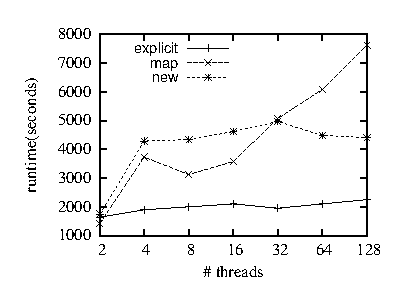
\includegraphics[width=80mm]{fig/rr.eps}
  \caption{The results of round-robin access pattern}
  \label{fig:rr_eval}
\end{figure}
\begin{SaveVerbatim}{ExplicitRoundRobinMonitor}
public class RoundRobinMonitor{
  final Lock mutex = new ReentrantLock();
  Condition[] conds;
  private int numProc;
  private int pid;

  public void access(int myId) {
    mutex.lock();
    while(pid != myId) {
      conds[pid].signal();
      conds[myId].await();
    }
    pid = (pid + 1) % numProc;
    conds[pid].signal();
    mutex.unlock();
  }
}
\end{SaveVerbatim}
\begin{SaveVerbatim}{RoundRobinMonitor}
public monitor class RoundRobinMonitor{
  private int numProc;
  private int numAccess;

  public void access(int myId) {
    await(pid == myId);
    pid = (pid + 1) % numProc;
  }
}
\end{SaveVerbatim}
\begin{figure}
  \centering
  \subfloat[Explicit-Signal] {
    \fbox{
      \BUseVerbatim[fontsize=\footnotesize]{ExplicitRoundRobinMonitor}
    }
    \label{subfig:rr_exam_exp}
  }
  \\
  \subfloat[Implicit-Signal] {
    \fbox{
      \BUseVerbatim[fontsize=\footnotesize]{RoundRobinMonitor}
    }
    \label{subfig:rr_exam_imp}
  }
  \caption{Round-Robin example}
  \label{fig:rbb_exp}
\end{figure}

%\subsection{Practical}
%Fig.~\ref{fig:dp_eval} shows the results of dining philosophers problem. The
%x-axis indicates the number of philosophers; the y-axis indicates the
%runtime in seconds. Every philosopher performed 100 eat operations with a
%randomly thinking time between 1 to 20 
%milliseconds. Fig.~\ref{fig:dp_eval} does not show the results of N-Condition 
%implementations since the results are much worse than other implementations. It
%takes around 10 minutes for 128 philosophers. The reason is that many waituntil
%statements with local predicate are used in this problem. Therefore, many
%conditional variables are created and removed at runtime. As can be seen, the
%other three approaches have the similar results. This phenomenon can be
%explained as follows. The thinking time is much larger than the synchronization 
%time in the monitor. Therefore, the runtime is dominated by the thinking time.
%%These results suggest that if applications do not have many operations to access
%%a monitor, the performance will not have much difference in implicit-signal and
%%explicit-signal monitor.
%
%
%\begin{figure}[ht!]
%  \centering
%  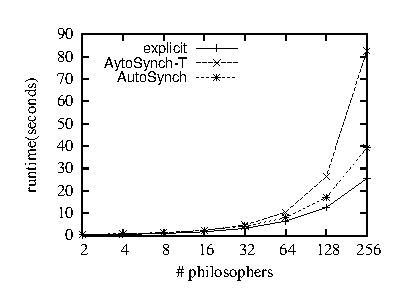
\includegraphics[width=80mm]{fig/dp.eps}
%  \caption{The results of dining philosophers problem}
%  \label{fig:dp_eval}
%\end{figure}

\begin{SaveVerbatim}{ExplicitTicketReadersWriters}
public class ReadersWritersMonitor {
  int rcnt;
  int tickets, serving;
  Lock mutex;
  Map<Integer, Condition> mapCondition;
  public void startRead() {
    mutex.lock();
    int ticket = tickets;
    tickets++;
    Condition cond = new Condition();
    mapCondition.put(ticket, cond);
    while(ticket != serving) {
      cond.await();
    }
    mapCondition.remove(ticket);
    rcnt++;
    serving++;
    mutex.unlock();
  }
  public void endRead() {
    mutex.lock();
    rcnt--;
    mutex.unlock();
  }
  public void startWrite() {
    mutex.lock();
    int ticket = tickets;
    tickets++;
    Condition cond = new Condition();
    mapCondition.put(ticket, cond);
    while(ticket != serving || rcnt != 0) {
      cond.await();
    }
    mapCondition.remove(ticket);
    mutex.unlock();
  }
  public void endWrite() {
    mutex.lock();
    serving++;
    mutex.unlock();
  }
}
\end{SaveVerbatim}
\begin{SaveVerbatim}{TicketReadersWriters}
public monitor class ReadersWritersMonitor {
  int rcnt;
  int tickets, serving;
  public void startRead() {
    int ticket = tickets;
    tickets++;
    await(ticket == serving);
    rcnt++;
    serving++;
  }
  public void endRead() {
    rcnt--;
  }
  public void startWrite() {
    int ticket = tickets;
    tickets++;
    await(ticket == serving && rcnt == 0);
  }
  public void endWrite() {
    serving++;
  }
}
\end{SaveVerbatim}

\begin{figure}
  \centering
  \subfloat[Explicit-Signal] {
    \fbox{
      \BUseVerbatim[fontsize=\footnotesize]{ExplicitTicketReadersWriters}
    }
    \label{subfig:rw_exam_exp}
  }
  \\
  \subfloat[Implicit-Signal] {
    \fbox{
      \BUseVerbatim[fontsize=\footnotesize]{TicketReadersWriters}
    }
    \label{subfig:rw_exam_imp}
  }
  \caption{Random Bounded-buffer example}
  \label{fig:rbb_exp}
\end{figure}
%\section{Discussions}
%\subsection{Comparison between different implementations}
%\subsection{Practical Issues} Need a big project to demonstrate 
%\section{Practical Case Study} Need a big project to demonstrate 

% An example of a floating figure using the graphicx package.
% Note that \label must occur AFTER (or within) \caption.
% For figures, \caption should occur after the \includegraphics.
% Note that IEEEtran v1.7 and later has special internal code that
% is designed to preserve the operation of \label within \caption
% even when the captionsoff option is in effect. However, because
% of issues like this, it may be the safest practice to put all your
% \label just after \caption rather than within \caption{}.
%
% Reminder: the "draftcls" or "draftclsnofoot", not "draft", class
% option should be used if it is desired that the figures are to be
% displayed while in draft mode.
%
%\begin{figure}[!t]
%\centering
%\includegraphics[width=2.5in]{myfigure}
% where an .eps filename suffix will be assumed under latex, 
% and a .pdf suffix will be assumed for pdflatex; or what has been declared
% via \DeclareGraphicsExtensions.
%\caption{Simulation Results}
%\label{fig_sim}
%\end{figure}

% Note that IEEE typically puts floats only at the top, even when this
% results in a large percentage of a column being occupied by floats.


% An example of a double column floating figure using two subfigures.
% (The subfig.sty package must be loaded for this to work.)
% The subfigure \label commands are set within each subfloat command, the
% \label for the overall figure must come after \caption.
% \hfil must be used as a separator to get equal spacing.
% The subfigure.sty package works much the same way, except \subfigure is
% used instead of \subfloat.
%
%\begin{figure*}[!t]
%\centerline{\subfloat[Case I]\includegraphics[width=2.5in]{subfigcase1}%
%\label{fig_first_case}}
%\hfil
%\subfloat[Case II]{\includegraphics[width=2.5in]{subfigcase2}%
%\label{fig_second_case}}}
%\caption{Simulation results}
%\label{fig_sim}
%\end{figure*}
%
% Note that often IEEE papers with subfigures do not employ subfigure
% captions (using the optional argument to \subfloat), but instead will
% reference/describe all of them (a), (b), etc., within the main caption.


% An example of a floating table. Note that, for IEEE style tables, the 
% \caption command should come BEFORE the table. Table text will default to
% \footnotesize as IEEE normally uses this smaller font for tables.
% The \label must come after \caption as always.
%
%\begin{table}[!t]
%% increase table row spacing, adjust to taste
%\renewcommand{\arraystretch}{1.3}
% if using array.sty, it might be a good idea to tweak the value of
% \extrarowheight as needed to properly center the text within the cells
%\caption{An Example of a Table}
%\label{table_example}
%\centering
%% Some packages, such as MDW tools, offer better commands for making tables
%% than the plain LaTeX2e tabular which is used here.
%\begin{tabular}{|c||c|}
%\hline
%One & Two\\
%\hline
%Three & Four\\
%\hline
%\end{tabular}
%\end{table}


% Note that IEEE does not put floats in the very first column - or typically
% anywhere on the first page for that matter. Also, in-text middle ("here")
% positioning is not used. Most IEEE journals/conferences use top floats
% exclusively. Note that, LaTeX2e, unlike IEEE journals/conferences, places
% footnotes above bottom floats. This can be corrected via the \fnbelowfloat
% command of the stfloats package.



\section{Conclusion} \label{sec:conclu}
The conclusion goes here. this is more of the conclusion

% conference papers do not normally have an appendix


% use section* for acknowledgement
\section*{Acknowledgment}


The authors would like to thank...
more thanks here


% trigger a \newpage just before the given reference
% number - used to balance the columns on the last page
% adjust value as needed - may need to be readjusted if
% the document is modified later
%\IEEEtriggeratref{8}
% The "triggered" command can be changed if desired:
%\IEEEtriggercmd{\enlargethispage{-5in}}

% references section

% can use a bibliography generated by BibTeX as a .bbl file
% BibTeX documentation can be easily obtained at:
% http://www.ctan.org/tex-archive/biblio/bibtex/contrib/doc/
% The IEEEtran BibTeX style support page is at:
% http://www.michaelshell.org/tex/ieeetran/bibtex/
%\bibliographystyle{IEEEtran}
% argument is your BibTeX string definitions and bibliography database(s)
%\bibliography{IEEEabrv,../bib/paper}
%
% <OR> manually copy in the resultant .bbl file
% set second argument of \begin to the number of references
% (used to reserve space for the reference number labels box)
\begin{thebibliography}{1}
\bibitem {bh05}
  P. A. Buhr and A. S. Harji, \emph{Implicit-Signal Monitors}. ACM 
  Transactions on Programming Languages and Systems ACM, 27(6):1270-1343, 
  Nov. 2005.

\bibitem {hoa74}
  C. A. R. Hoare, \emph{Monitors: an operating system structuring concept}, 
  Commun.~ACM 17, 10(Oct. 1974), 549-557.

\end{thebibliography}




% that's all folks
\end{document}


